\chapter{ELEMENTARY SUBSTITUTION SYSTEMS}

\section{GENERAL}

\subsection{Fundamental Nature of Substitution Methods. Cipher Systems and Code Systems}

Methods now to be described differ from those above in that elements
or textual units composing the original plain text retain their relative
positions, but not their identities, and are replaced by other elements or
textual units so that the external form of the writing is cryptographic in
nature. For this reason these methods are called substitution methods.
They may deal with individual letters, pairs of letters, sets of letters in
regular groups, syllables, whole words, phrases, and sentences. Substitution methods may accordingly be subdivided into letter methods, syllable
methods, and word methods, as in the case of transposition methods;
but such a classification is a rather arbitrary one and is not based on the
nature, form, or external appearance of the cryptographic text. For
example, a substitution method dealing with single letters of the plain text
may not involve their replacement by other single letters. In some cases
whole words may be used to replace single letters. Outwardly, such a
cryptogram gives the appearance of dealing with words, but its internal
nature is quite clear: single-letter substitution has been effected. The
classification indicated is, nevertheless, a useful one. When the cryptographic process involves the treatment of individual letters or pairs of
letters, and only exceptionally the treatment of syllables or whole words,
the method is known as a substitution cipher system; and when the
process involves the treatment of whole words, phrases, or sentences, and
only exceptionally the treatment of individual letters, groups of letters,
or syllables, the method is known as a code system, because it usually
necessitates the use of a code book.

\subsection{Nature of Alphabets}

\mypara The simplest kind of substitution cipher is that which is known in
literature as Julius Caesar’s Cipher, but which, as a matter of fact, was a
favorite long before his day. In this cipher each letter of the text of a
message is replaced by the letter standing the third to the right of it in
the ordinary alphabet; the letter A is replaced by D, the letter B by E,
and so on. The word CAB becomes converted into F DE which is cipher.

\mypara The English language is written by means of 26 simple characters
called letters which, taken together and considered as a sequence of symbols, constitute the alphabet of the language. Not all systems of writing
are of this nature. Chinese writing is composed of about 44,000 complex
characters, each representing one sense of a word. Whereas English
words are composite or polysyllabic and may consist-of one to eight or
more syllables, Chinese words are all monosyllables and each .mono-
syllable is a word. Written languages of the majority of other civilized
peoples of today are, however, alphabetic and polysyllabic in construction,
so that principles discussed here apply to all of them.

\mypara The letters composing the English alphabet used today are the results
of a long period of evolution, the complete history-of which may never
fully be known. They are conventional symbols representing elementary
sounds, and any other simple symbols, so long as the sounds which they
represent are agreed upon by those concerned, will serve the purpose
equally well. If taught from early childhood that the symbols \$, *, and
@ represent the sounds “Ay,” “Bee,” and “See,” respectively, the
combination \@\$* would still be pronounced CAB, and would, of course,
have exactly the same meaning as before; or suppose that two persons
have agreed to change the sound values of the letters, F, G, and H, and
after long practice have become accustomed to pronouncing them as
“Ay,” “Bee,” and “See,” respectively. They would then write the “word"
HFG, pronounce it CAB, and see nothing strange whatever in the
matter. But to others not party to their arrangements HFG constitutes
cipher. The combination of sounds called for by this combination of symbols is perfectly intelligible to the two who have adopted the new sound
values for those symbols and therefore pronounce HFG as CAB, but
HFG is utterly unpronounceable and wholly unintelligible to others who
are reading it according to their own long established sound-symbol basis.
It would be stated that there is no such word as HFG, which would
mean merely that the particular combination of sounds represented by
this combination of letters has not been adopted by convention to represent a thing or an idea in the English language. Thus it is seen that, in
order for the written words of a language to be pronounceable and
intelligible to all who speak that language, it is necessary, first, that the
sound values of the letters or symbols be universally understood and
agreed upon and, secondly, that the particular combination of sounds
denoted by the letters should have been adopted to represent a thing or
an idea. Spoken plain language consists of vocables; that is, combinations and permutations of elementary speech—sounds which have by long
usage come to be adopted and recognized as representing definite things
and ideas. Written plain language consists of words; that is, combina-
tions and permutations of simple symbols, called letters, which represent
visually and call forth vocally the elementary speech-sounds of which
the spoken language is composed.


\mypara It is clear also that in order to write a polysyllabic language with
facility it is necessary to establish and to maintain by common agreement
or convention, equivalency between two sets of elements, first, a set of
elementary sounds and, second, a set of elementary symbols to represent the sounds. When this is done the result is what is called an alphabet,
a word derived from the names of the first two letters of the Greek
alphabet, “alpha” and “beta.”

\mypara Theoretically, in an ideal alphabet each symbol or letter would
denote only one elementary sound, and each elementary sound would
invariably be represented by the same symbol. But such an alphabet
would be far too difficult for the average person to use. It has been
conservatively estimated that a minimum of 100 characters would be
necessary for English alone. Attempts toward producing and introducing
into usage a practical, scientific alphabet have been made, one being that
of the Simplified Spelling Board in 1928, which advocated a revised
alphabet of 42 characters. Were such an alphabet adopted into current
usage, in books, letters, telegrams, etc., the flexibility of cryptographic
systems would be infinitely extended and the difficulties set in the path
of the enemy cryptanalysts vastly increased. The chances for its adoption
in the near future are, h0wever, quite small. Because of the continually
changing nature of every living language, it is doubtful whether an
original perfect alphabet could, over any long period of time, remain
so and serve to indicate with great precision the exact sounds which it
was originally designed to represent.

\subsection{Normal Alphabets and Cipher Alphabets}

\mypara In the study of cryptography the dual nature of the alphabet be—
comes apparent. It consists of two parts or components, (1) an arbi-
trarily arranged sequence of symbols.

\mypara The normal alphabet for any language is one in which these two
components are the ordinary sequences that have been definitely fixed by
long usage or convention. The dual nature of our normal or everyday
alphabet is often lost sight of. When we write A, B, C, . . . we really
mean:

\begin{verbatim}
Sequence of sounds: "Ay" "Bee" "See"

Sequence of symbols: A    B     C
\end{verbatim}

Normal alphabets of different languages vary considerably in the number
of characters composing them and the arrangement or sequence of the
characters. The English, Dutch, and German alphabets each have 26,
the French 25, the Italian 21, Spanish 27 (including the digraphs ch and
ll), Russian 31. The Japanese language has a syllabary consisting of
72 syllabic sounds, to express which 48 characters are employed.

\mypara A cipher alphabet or a substitution alphabet, as it is sometimes
called, is one in which the elementary speech-sounds are represented by
characters other than those representing them in the normal alphabet.
These characters may be letters, figures, signs, symbols, or combinations
of them.

\mypara A more technical definition of a familiar cipher may now be given:
When the plain text of a message is converted into encrypted text by the
use of one or more cipher alphabets, the resultant cryptogram constitutes
a \textit{substitution cipher}.

\subsection{Two Components of an 'Alphabet}

It is convenient to designate that component of a cipher alphabet con-
stituting the sequence of speech—sounds the plain component, and the
component constituting the sequence of symbols the cipher component. If
the plain component is omitted in a cipher alphabet, the latter is understood to be the normal sequence. For brevity and clarity, a letter of the
plain text, or of the plain component of a cipher alphabet, is designated
by suffixing a small letter “p” to it: A, means A of the plain text, or of
the plain component of a cipher alphabet. Similarly, a letter of the cipher
text, or of the cipher component of a cipher alphabet, will be designated
by suffixing a small letter “c” to it: Xc means X of the cipher text, or
of the cipher component of a cipher alphabet. The expression A,. = Xe
means that A of the plain text, or A of the plain component of a cipher
alphabet, is represented by X in the cipher text, or by X in the cipher
component of a cipher alphabet.

\subsection{Standard and Mixed Cipher Alphabets}

In the arrangement or sequence of letters forming its cipher compo-
nent, cipher alphabets arc of two kinds:

\begin{enumerate}[label=\alph*]
\item Standard cipher alphabets, in which the sequence of letters in the
cipher component is the same as the normal, but reversed in direction or
shifted from its normal point of coincidence with the plain component.

\item Mixed cipher alphabets, in which the sequence of letters or char-
acters in the cipher component is no longer the same as the normal in its
entirety.
\end{enumerate}

\subsection{Enciphering and Deciphering Alphabets}

All cipher alphabets may be classified on the basis of their arrange-
ment as enciphering or deciphering alphabets. An enciphering alphabet is
one in which the sequence of letters in the plain component coincides with
the normal sequence, and is arranged in that manner for convenience
in encipherment. In a deciphering alphabet the sequence of letters in the
cipher component coincides with the normal, for convenience in deciphering. For example, in figure 9, (a) shows a mixed cipher alphabet
arranged as an enciphering alphabet; (b) shows the corresponding
deciphering alphabet. An enciphering alphabet and its corresponding
alphabet present a verse and inverse relationship to each other. To invert
a deciphering alphabet is to write the corresponding enciphering alphabet;
to invert an enciphering alphabet is to write the corresponding deciphering alphabet.

\begin{textfigure}
\textit{Enciphering Alphabet}

        \begin{verbatim}
(a)    Plain:  ABCDEFGHIJKLMNOPQRSTUVWXYZ
       Cipher: JKQVXZWESTRNUIOLGAPHCMYBDF
        \end{verbatim}

        \textit{Deciphering Alphabet}

        \begin{verbatim}
(b) Cipher: ABCDEFGHIJKLMNOPQRSTUVWXYZ
    Plain:  RXUYHZQTNABPVLOSCKIJMDGEWF
        \end{verbatim}
        \caption{Figure 9}
\end{textfigure}

\section{MONOALPHABETIC SUBSTITUTION SYSTEMS}

\subsection{Single-Alphabet Substitution}

If a message is enciphered, letter—for—letter, by using one cipher
alphabet which has been drawn up for the purpose, the resulting crypto-
gram is said to be enciphered by a single alphabet and to-be a single-
alphabet, or monoalphabetic, substitution cipher. More complex ciphers
may use several alphabets in the enciphering of a single message. When
two or more cipher alphabets are used, the resulting cryptogram is said
to be a polyalphabetic cipher.

\subsection{Standard Alphabet Ciphers}

\mypara Standard cipher alphabets are of two sorts:
\begin{enumerate}
\item Direct standard, in which cipher component is the normal
sequence but shifted to the right or left of its point of coincidence in the normal alphabet. Example:

\longrightarrow
\begin{verbatim}
Plain:   ABCDEFGHIJKLMNOPQRSTUVWXYZ
Cipher : QRSTUVWXYZABCDEFGHIJKLMNOP
\end{verbatim}
\longrightarrow

It is obvious that the cipher component can be applied to the
plain component at any one of 26 points of coincidence, but
since the alphabet that results from one of these applications
coincides exactly with the normal alphabet, a series of only
25 (direct standard) cipher alphabets results from the shifting
of the cipher component.

\item Reversed standard, in which the cipher component is also the
normal sequence but runs in the opposite direction from the
normal. Example:

\begin{verbatim}
->
Plain:  ABCDEFGHIJKLMNOPQRSTUVWXYZ
Cipher: QPONMLKJIHGFEDCBAZYXWVUTSR
<-
\end{verbatim}

Here the cipher component can be applied to the plain com-
ponent at any of 26 points of coincidence, each yielding a
different cipher alphabet. There is in this case, therefore, a
series of 26 (reversed standard) cipher alphabets.
\end{enumerate}

\mypara It is often convenient to refer to or designate one of a series of
cipher alphabets without ambiguity or circumlocution. The usual method
is to indicate the particular alphabet to which reference is made by citing
a pair of equivalents in that alphabet. For example, the reversed alphabet
above, one of a series of 26 related alphabets, may be designated as that
in which Ln = Fc or Wp = Uc. But the most common basis of reference is the letter which represents the first or initial letter of the plain
component, usually A,. Thus, the key for the cipher alphabet just
referred to, as well as that preceding it, is A, = Qc, and it is said that the
key letter for the cipher alphabet is Qc.

\subsection{Reciprocal Alphabets}

\mypara The cipher alphabet in paragraph 42a (2) is also a reciprocal
alphabet; that is, the equivalents show reciprocity and are reversible or
reciprocal in pairs. For example, in the alphabet referred to, Ap = Qc
and 9,. =Ac ; B, = PC and Pp = Be, etc. The reciprocity exists throughout the alphabet and is a result of the method by which it was formed.

\mypara A series of related reciprocal alphabets may be derived by juxtaposing at all possible points of coincidence two components which are identical but progress in opposite directions. This holds regardless of whether
the components are composed of an even or an odd number of elements.
The reciprocal alphabet (par. 42a (2)) is one of such a series of 26
alphabets.

\mypara A single or isolated reciprocal alphabet may be produced in one of
two ways:

\begin{enumerate}
\item By constructing a complete reciprocal alphabet by arbitrary or
random assignments of values in pairs. That is, if A, is made
Kc, then K,, is made Ac; if B, is made Re, then R, is made Be,
and so on. If the two components thus constructed are slid
against each other no additional reciprocal alphabets will be
produced.

\item By juxtaposing a sequence comprising an even number of
elements against the same sequence shifted exactly half way to
the right (or left), as seen below;

\begin{verbatim}
ABCDEFGHIJKLMNOPQRSTUVWXYZABCDEFGHIJKLMNOPQRSTUVWXYZ
             ABCDEFGHIJKLMNOPQRSTUVWXYZ
\end{verbatim}
\end{enumerate}

\mypara A reciprocal alphabet is an inverse alphabet, since it may serve
either as an enciphering or deciphering alphabet.

\subsection{Procedure in Enciphermenf and Decipherment}

\mypara When a message is enciphered monoalphabetically, that is, by
means of a single cipher alphabet, letters of the text are replaced by the
equivalents in the cipher alphabet selected by prearrangement. Example:

Message: THREE MACHINE GUNS CAPTURED.

Enciphering Alphabet: Reversed Standard, AI) = D.,.

\begin{verbatim}
Plain :  ABCDEFGHIJKLMNOPQRSTUVWXYZ
Cipher : DCBAZYXWVUTSRQPONMLKJIHGFE
\end{verbatim}

Letter-for-letter encipherment:

\begin{verbatim}
THREE MACHINE GUNS CAPTURED
KWMZZ RDBWVQZ XJQL BDOKJMZA
\end{verbatim}

The cipher text is then grouped in fives and the indicator letter D\footnote{If this or any such similar convention has been agreed upon by the correspondents}
inserted as the initial letter of the first group (or any other prearranged
group).

Cryptogram:
\begin{textfigure}
        \begin{verbatim}
DKWMZ ZRDBW VQZXJ QLBD-O KJMZA
        \end{verbatim}
        \caption{Figure 10}
\end{textfigure}

\mypara The procedure in decipherment is merely the reverse of that in
encipherment. The initial letter of the message, D, indicates A, = Dc in
the cipher alphabet. The deciphering alphabet is therefore as follows:

\begin{verbatim}
Cipher : ABCDEFGHIJKLMNOPQRSTUVWXYZ
Plain :  DCBAZYXWVUTSRQPONMLKJIHGFE
\end{verbatim}

The message deciphers thus:
\begin{verbatim}
Cipher: (D) KWMZ ZRDBW VQZXJ QLBDO KJMZA
Plain:      THRE EMACH INEGU NSGAP TURED
\end{verbatim}

The deciphering clerk rewrites the text in word lengths:
THREE MACHINE GUNS CAPTURED

\mypara When a mixed alphabet is used, the enciphering and deciphering
processes are the same as those described under a and b above. For
speed in cryptographing, the cipher alphabet is prepared in the form of
an enciphering alphabet, and for speed in decryptographing, in the form
of a deciphering alphabet.

\section{TYPES OF MIXED CIPHER ALPHABETS}
\subsection{Systematically Mixed Cipher Alphabets}

It will be recalled that in a mixed cipher alphabet the sequence of
letters or characters in the cipher component does not correspond to the
normal sequence. 'There are various methods of mixing up the letters of
the cipher component, and those which are based upon a scheme that is
systematic in its nature are very useful because they make possible the
derivation of one or more mixed sequences from any easily remembered
word or phrase, and thus do not necessitate the carrying of written
memoranda. They are called systematically mixed cipher alphabets.

\subsection{Key-word Mixed Alphabets}

\mypara One of the simplest types of systematically \textit{mixed cipher alphabets}
is the key-word mixed alphabet. The cipher alphabet consists of a key
word or phrase (with repeated letters, if present, omitted after their first
occurrence), followed by the letters of the alphabet in their normal
sequence (with letters already occurring in the key, of course, omitted).
Example, with GOVERNMENT the key word:
\begin{verbatim}
Enciphering alphabet....  { Plain:  ABCDEFGHIJKLMNOPQRTSUVWXYZ
                            Cipher: GOVERNMTABCDFHIJKLPQSUWXYZ
\end{verbatim}

\mypara Mixed alphabets formed by including all repeated letters of the key
word or key phrase were common in Edgar Allan Poe’s day but are
impractical because they make decipherment diflicult.

\begin{verbatim}
Enciphering alphabet.... { Plain:  ABCDEFGHIJKLMNOPQRSTUVWXYZ
                           Cipher: NOWISTHETIMEFORALLGOODMENT
Deciphering alphabet.... { Cipher: ABCDEFGHIJKLMNOPQRSTUVWXYZ
                           Plain:  P  VHMSGD  QKAB  OEF  C
                                       L   J  RWYN    I
                                       X         T    Z
                                                 U
\end{verbatim}

The average cipher clerk would have considerable difficulty in decryptographing a cipher group such as TOOET, each letter of which has three
or more equivalents, and from which the plain-text words (N) INTH,
. .FT THI (S), IT THI . . . , etc., can be formed on decipherment.

\mypara An example of a key-word mixed alphabet is shown in figure 9,
where, in its enciphering form, the cipher component presmts to the
experienced eye the skeleton of the key upon which the alphabet is
based: WESTERN UNION TELEGRAPH COMPANY. Any easily
remembered word, phrase, or sentence may be used. The starting point
of the sequence, when used as a cipher component, may be indicated
in the usual manner. For example, in the alphabet referred to, the
alphabet key is A, = In. Two or more correspondents using the prearranged key, WESTERN UNION TELEGRAPH COMPANY,
would obtain the same disarranged sequence; when this sequence is to
form the cipher component of a cipher alphabet, the prearranged key
letter A1, = Jo would result in giving each correspondent exactly the
same cipher alphabet. The key words or phrases need not consist of any
definite number of letters, but it is advisable to use for keys such words
or phrases as will most thoroughly disarrange the normal sequence. (See,
in this connection, par. 26.) A key-word mixed alphabet will manifest
the key word or parts of it only when the alphabet is in the form of
an enciphering alphabet. Note that alphabet (b) of figure 9 no longer
gives any external evidence of having been derived from the phrase
WESTERN UNION TELEGRAPH COMPANY.

\subsection{Transposition-mixed Alphabets}

\mypara It is possible to disarrange the sequence even more thoroughly by
applying a simple method of transposition to the key—word sequence
as if it were a message. An example is illustrated in figure 11.

Key word:
\begin{textfigure}
        \begin{verbatim}
                TELPHONY
        \end{verbatim}

(a) Simple columnar transposition:
    \begin{verbatim}
                TELPHONY
                ABCDFGIJ
                KMQRSUVW
                XZ
    \end{verbatim}

Mixed sequence :
        \begin{verbatim}
        TAKXEBMZLCQPDRHFSOGUNIVYJW
    \end{verbatim}

(b) Numerical key, columnar transposition:

        \begin{verbatim}
            7-1-5-6-2-5-4-8
            T E L P H O N Y
            A B C D F G I J
            K M Q R S U V W
            X Z
        \end{verbatim}

Mixed sequence :
        \begin{verbatim}
        EBMZHFSLCQNIVOGUPDRTAKXYJW
        \end{verbatim}
        \caption{Figure 11}
\end{textfigure}

\mypara The last two systematically mixed cipher alphabets are transposition-mixed alphabets. Almost any of the methods of transposition
described in sections IV and V of this chapter may be applied to them.

\subsection{Decimafion Method of Forming Mixed Alphabets}

Another simple method of forming a mixed alphabet is the decimation
method. In this method, letters in the normal alphabet, or in a key—word
mixed alphabet, are “counted off” according to a selected odd interval.
As each letter is decimated—that is, eliminated from the basic alphabet
by counting off—it is entered in a separate list to form the sequence of
the mixed alphabet. For example, to form a mixed alphabet by this
method from an alphabet based on the key phrase SING A SONG OF
SIX PENCE with 7 the interval selected, proceed as follows:

\begin{enumerate}[label=\alph*]
\item Key-word (or basic) alphabet:

        \begin{verbatim}
SINGAOFXPECBDHJKLMQRTUVWYZ
        \end{verbatim}

\item When the letters are counted off by 7’s frOm left to right, F will
be the first letter arrived at, H the second, T the third:


\begin{figure}[h]
 \centering
 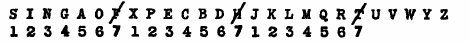
\includegraphics[width=0.7\textwidth, natwidth=470,natheight=43]{Chapter3_FigB.eps}
 \caption{Fig. B}
\end{figure}

These letters are entered in a separate list (F first, H second, T third,
etc.) and eliminated from the key—word alphabet.

\item When the end of the key-word alphabet is reached, return to the
beginning, skipping the letters already eliminated:
\begin{figure}[h]
 \centering
 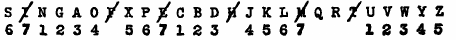
\includegraphics[width=0.7\textwidth, natwidth=470,natheight=43]{Chapter3_FigC.eps}
 \caption{Fig. C}
\end{figure}

\item Mixed alphabet.

        \begin{verbatim}
FHTIEMZPQNDWCVBSLXAGOKYJRU
        \end{verbatim}
\end{enumerate}

\subsection{Random-Mixed Alphabets}

Practical considerations, of course, set a limit to the complexities that
may be introduced in constructing systematically mixed alphabets.
Beyond a certain point there is no object in further mixing. The greatest
amount of mixing by systematic processes will give no more security
than that resulting from mixing the alphabet by random selection, such
as by putting the 26 letters in a box, thoroughly shaking them up, and
then drawing the letters out one at a time. Whenever the laws of chance
operate in the construction of a mixed alphabet, a thorough disarrangement is bound to be produced. Random-mixed alphabets give more
Cryptographic security than do the less complicated systematically mixed
alphabets because they afford no clues to positions of letters, given the
positions of a few of them. Their chief disadvantage is that they must be
reduced to writing, since they cannot readily be remembered, nor can
they be reproduced at will from an easily remembered key word.

subsection{Number of Single Alphabets Available from a Basic Alphabet}

It is obvious that the cipher component of a cipher alphabet may be
shifted or slid against the plain component at 26 points of contact so as
to produce a series of different enciphering alphabets. For example, the
mixed sequences given under (b) of figure 11, when used as a cipher
component, yields the following two of a series of 26 cipher alphabets:

\begin{center}
\textit{Enciphering Alphabets}
\end{center}

\begin{verbatim}
(1) Plain:   ABCDEFGHIJKLMNOPQRSTUVWXYZ
    Cipher : EBMZHFSLCQNIVOGUPDRTAKXYJW

(2) Plain:   ABCDEFGHIJKLMNOPQRSTUVWXYZ
    Cipher : WEBMZHFSLCQNIVOGUPDRTAKXYJ
\end{verbatim}

The message DAILY REPORT NOT RECEIVED YET would be
enciphered by the first alphabet as:

\begin{verbatim}
Plain:  DAILY REPOR TNOTR ECEIV EDYET
Cipher: ZECIJ DHUGD TOGTD HMHCK HZJHT
\end{verbatim}

and by the second alphabet as:
\begin{verbatim}
Plain:  DAILY REPOR TNOTR ECEIV EDYET
Cipher: MWLNY PZGOP RVORP ZBZLA ZMYZR
\end{verbatim}

Externally the two cryptograms seem different except in length. The two
enciphering alphabets present the same sequence in the cipher component, but this entirely disappears in the corresponding deciphering
alphabets, which are as follows:

\begin{center}
\textit{Deciphering Alphabets}
\end{center}

\begin{verbatim}
(1) Cipher: ABCDEFGHIJKLMNOPQRSTUVWXYZ
    Plain:  UBIRAFOELYVHCKNQJSGTPMZWXD
\end{verbatim}
\begin{verbatim}
(2) Cipher: ABCDEFGHIJKLMNOPQRSTUVWXYZ
    Plain:  VCJSBGPFMZWIDLORKTHUQNAXYE
\end{verbatim}

It is possible to write the same message in 25 different external forms,
each using a different cipher alphabet of a series derivable from a
basic sequence. The basic sequence or alphabet in such a case is often
called a primary sequence or a primary alphabet; derived alphabets
are called secondary alphabets. In producing secondary alphabets the
basic sequence must be juxtaposed and slid against itself, or against
the normal sequence, or against another mixed sequence. In all cases
secondary alphabets form a series of alphabets that are interrelated and
that either directly or indirectly manifest relationships which are important from a cryptanalytic point of view. It should be clear now that
by means of a single, prearranged, secret word it is possible for two
correspondents to send a whole set of messages all in different mixed
alphabet, or to use a different alphabet for each of 26 consecutive days.

\subsection{Miscellaneous Types of Cipher Alphabets}

\mypara The cipher alphabets shown thus far have used only letters, but
alphabets in which the cipher component consists of figures, or groups
of figures, are not uncommon in military cryptography. Cipher alphabets
using signs and symbols are not suitable for military cryptography because they can neither be telegraphed nor telephoned with any degree
of accuracy, speed, or facility. Since there are but ten digits it is obvious
that, in order to represent a camplete alphabet in figure ciphers, combinations of at least two digits are necessary. The simplest kind of such
an alphabet is that in which A\textsubscript{\textit{p}} = 01, B\textsubscript{\textit{p}} = 02,. . . Z\textsubscript{\textit{p}} = 26.

\begin{figure}[h]
 \centering
 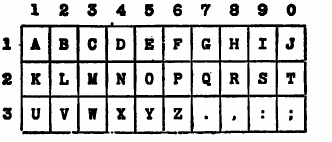
\includegraphics[width=0.7\textwidth, natwidth=332,natheight=142]{Chapter3_Figure12.eps}
 \caption{Figure 12}
\end{figure}

\mypara Instead of a simple alphabet of the preceding type, it is possible
to use a simple diagram of the type shown in figure 12. Here the digits
at the side and top of the rectangle are used to designate, according to
the coordinate system, the cell occupied by each letter and punctuation
mark within the rectangle. When used for such purposes, the figures (or
letters) constituting coordinate elements are referred to as raw and
column indicators. It is usually necessary to agree beforehand upon
which indicator will be given as the first half of the equivalent for a
letter, the row indicator or the column indicator, in order to avoid
ambiguity or error. In all of the systems to be described here, the row
indicator will always form the first half of an equivalent. Accordingly
in figure 12, the letter A, = 11, B, = 12, and so forth.

\mypara A variation of the foregoing diagram is exemplified in figure 13.
Here, letters of the alphabet are inserted in the 25 cells of a large square,
I and I being written together in one cell. Then a key word of five let-
ters is applied to the top of the large square and the same or a differ-
ent key word is applied to the side of the square to form column and row
indicators. In figure 13, for example, Sp = TI; W: = EH; etc.

\begin{figure}[h]
 \centering
 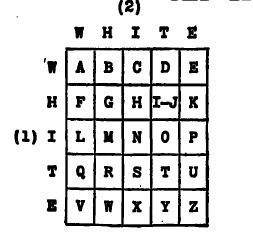
\includegraphics[width=0.7\textwidth, natwidth=253,natheight=241]{Chapter3_Figure13.eps}
 \caption{Figure 13}
\end{figure}

The message RAIDERS HAVE GONE is enciphered thus:

\begin{verbatim}
Plain:   R  A  I  D  E  R  S  H  A  V  E  G  O  N  E
Cipher: TH WW HT WT WE TH TI HI WW EW WE HH IT II WE
\end{verbatim}

The cryptogram is then transmitted in groups of five letters:
\begin{verbatim}
Cryptogram: THWWH TWTWE THTIH IWWEW WEHHI THWE
\end{verbatim}

\mypara In these two systems just described,

\begin{enumerate}
\item The letters of the alphabet within the square or rectangle may
be fixed in a mixed sequence, either systematically or random-
mixed sequences being possible.

\item The column and row indicators may be the same, or different;
when letters are used they may form a key word or they may
not; the key words, if formed, may be identical or nonidentical.
\end{enumerate}

\mypara When letters are used as column and row indicators, they may be
selected so as to result in producing cipher text that resembles “made-up
words,” that is, words composed of regular alternations of vowels and
consonants. For example, if in figure 13 the row indicators consisted of
the vowels A E I O U in this sequence from the top down, and the
column indicators consisted of the consonants B C D F G in this
sequence from left to right, the word RAIDS would be enciphered as
OCABE FAFOD, which very closely resembles code of the type formerly called artificial code language. Such a system may be called a
false, or pseudo-code system.\footnote{Prior to 1934, International Telegraph Regulations required code words of five letters to contain It least one vowel and code words of ten letters to contain at least three vowels. The Madrid Conference held in 1932 amended these regulations to permit the use of code groups containing any combination of letters. These unrestricted eude groups were authorized for use after 1 January 1934.}

\section{MONOALPHABETIC SUBSTITUTION WITH VARIANTS}

\subsection{Purpose of Providing Variant Values}

The individual letters composing ordinary intelligible plain text are
used with varying frequencies; some, such as (in English) E, 'l‘, R, I,
and N, are used much more often than others, such as J, K, Q, X, and Z.
In fact, each letter has a characteristic frequency by means of which
definite clues are afforded in the solution of simple substitution ciphers.
This has led cryptographers to devise methods for disguising, sup—
pressing, or eliminating the characteristic frequencies manifested by the
letters of cryptograms produced by simple monoalphabetic substitution.
One such method is that in which the letters of the plain component of
the cipher alphabet are assigned two or more equivalents in the cipher
component and they are, for this reason, called variant values. In some
cases the letters of the plain component receive numbers of variant
.values, or variants, in proportion to their normal frequencies; in other
cases, all the letters receive equal numbers of variant values, determined
by the total number available.

\subsection{Figure Ciphers with Variant Values}

\mypara The use of figures in pairs as substitution equivalents makes available a total of 100 different pairs, those from 00 to 99. They may all
be used in a complete system, or only certain ones may be selected, as
prearranged.

\mypara One of the most common varieties of ciphers using all the pairs of
digits is that in which the alphabet is reduced to 25 letters (by making
1 and J interchangeable or by eliminating a letter such as Q), and each
letter is assigned four values which may be used at will. The assignment
of values may be based upon a key word of four letters, each of which
designates the starting points of a normal sequence of 25 numbers. An
example is shown in figure 14, wherein the key word is TRIP. This
means that in the first set of numbers, 01 to 25, the first number, 01, is
assigned to the letter T; in the second set, from 26 to 50, the first num-
ber, 26, is assigned to the letter R; in the third set, from 51 to 75, the
first number, 51, is assigned to the letter I; finally, in the last set, from
76 to 00, the first number, 76, is assigned to the letter P.

The letter Ap may be represented by any one of four equivalents, 08,
35, 68, and 87; the letter B, by 09, 36, 69, 88; and so on. The equivalent
used in any particular instance is selected at random, so that the word
.CAB may be represented in cipher by any one of a total of 64 combina-
tions, such as 10—08—09, 70—35—09, 37—08—69, etc. In the final cryptogram
the figures may be run together in groups of five. The cipher group
10080, on deciphering, would be split up into 10-08—0.

\begin{textfigure}
        \begin{verbatim}
        A-08 35 68 87  I-J-16 43 51 95    S-25 27 50 79
        B-09 36 69 88    K-17 44 52 96    T-01 28 61 80
        C-10 37 7O 89    L-18 45 53 97    U-02 29 62 81
        D-11 38 71 90    M-19 46 54 98    V-03 30 63 82
        E-12 39 72 91    N-2O 47 55 99    W-04 31 64 83
        F-13 40 73 92    O-21 48 56 00    X-05 32 55 84
        G-14 41 74 93    P-22 49 57 76    Y-06 33 55 85
        H-I5 42 75 94    Q-23 50 58 77    Z-07 34 57 86
                         R-24 26 59 78
        \end{verbatim}
        \caption{Figure 14}
\end{textfigure}

\mypara In this case, within each set of 25 the numbers progress serially,
each set being treated as a ring or circle. It is of course possible to mix
the sequence to destroy this serial progression, thus giving four mixed
alphabets which can be used at random.
\mypara Another variation is to assign each letter a set of numbers in accordance with its relative frequency in ordinary English, so that each of
the most frequently used letters such as E, T, R, I, and N will have
perhaps seven or eight different equivalents, whereas letters of low frequency such as J, K, Q, X, and Z will each have but one equivalent.

\subsection{Use of Rectangles to Provide Variant Values}

\mypara Instead of drawing up alphabets as in figure 14, it is possible to use
the diagram shown in figure 12, but with several variant digits as row
indicators instead of a single digit for each row. For example, the row
indicators may be of the following arrangements:

\begin{verbatim}
 1-6-7    1-2-3   1-2-3   5-4-3
 2-5-8    4-5-6   8-9-4   6-9-2
 3-4-9    7-8-9   7-6-5   7-8-1, etc.
\end{verbatim}

Thus, if the first arrangement is used, A, would have the equivalents 11,
61, 71; B,,, 12, 62, 72; etc. The word RUN might be represented by
any one of 27 different combinations, such as 28—31—24, 28—91—54, etc.

\mypara A variation of the foregoing system is that in which, by use of a
diagram of the type shown in figure 13, a number of different letters are
applied to each row and column, or Z-figure numbers may be used for
this purpose. In this case a series of as many as 50 pairs of digits may be
used as row indicators, and another series of 50 pairs as the column
indicators.

\mypara The use of variants lends itself to application in a pseudo-code system such as described in paragraph 51e. It presents many possibilities for variation, with or without key words, with one or more alphabets distributed within the square or rectangle, with alphabets extended to include figures, punctuation signs, common syllables and words, etc. Some
times pseudo-code is encountered when the groups of a numerical cipher
system (or a figure-code system) are converted into letters, in order to
make the cryptographic text conform to certain telegraph regulations
and thus have the message accorded a more favorable rate of charge (sec.
II, ch. 4). Thus, a group such as 0125784256 might be converted into the
group BAFOSULAFE. If the conversion table "is irregular in its construction and is kept secret, this adds an encipherment step to the system.

\subsection{Disadvantages of Monoalphabotic Substitution with Variants}

The obvious disadvantage of all such methods discussed in the preceding paragraph is that the cryptographic text is exactly twice as long as
the original plain text. Furthermore, there is no compensating advantage
from the standpoint of cryptographic security. When methods are such
that the cipher equivalents are passed through another process which returns the cipher text to a length identical with that of the equivalent plain
text, they are usually too complicated, too slow, and too subject to error
to be practical. They are often the result of combining substitution and
transposition processes in one system. Methods which substitute three
or more characters for one letter of the original text are not at all practical for military cryptography.

\section{POLYALPHABETIC SUBSTITUTION SYSTEMS}

\subsection{Monoalphabetic and Polyalphabetic Substitution}

\mypara In the substitution methods thus far discussed it has been noted that
only one cipher alphabet is used in the encipherment of a message, and
that as a class they constitute the type of system designated as monoalphabetic substitution. It is true that in certain of the systems monoalphabetic substitution with variant equivalents takes place, there are two
or more complete alphabets involved and that these systems may, therefore, with apparently good reason be designated as polyalphabetie substitution. This designation, however, will be seen to be somewhat inaccurate when cases of true polyalphabetie substitution come to be studied.
The real or essential difference between the two systems may best be
made clear by setting forth the primary object in each case.

\mypara In monoalphabetic substitution with variant values, the object of
having difl-‘erent sets of equivalents is to suppress so far as possible by
simple methods the characteristic frequencies of letters. One such method
consists in merely providing one or more different values as cipher
equivalents of the same plain-text letter, of a few different values as 
equivalents of some of the high-frequency letters. Now there are certain
conditions inherent in the method itself, conditions which cannot here be
indicated, that result in producing in the cryptograms certain definite
clues leading to the rapid establishment, in cryptanalysis, of the equivalence of different variant values. Furthermore, in these systems the varying or alternative equivalents for plain—text letters are subject to the free
choice and caprice of the encipherer. If he is careful and conscientious
in the work he will actually make use of all the variant values afforded
by the system; but if he is slip—shod and hurried in his work, he will use
the same equivalent repeatedly rather than take pains and time to refer
to his charts, tables, or diagrams to find variants. The result is that the
cryptograms based upon these methods are open to easy solution, even
when the basic methods are such as would make a solution difficult without the interception of carelessly enciphered messages. What is necessary
is a system in which there is established a definite procedure for auto
matically shifting or changing the cipher alphabets employed in the encipherment of a single message; a method which within certain limits is
beyond the momentary whims of cipher clerks, and which to a higher
degree makes difficult the establishment of the equivalency of different
cipher values. These are the objects of true polyalphabetic substitution
systems. The number of such systems is large. Therefore, it will be possible to describe only a few of the more common or typical examples of
methods practicable for military use.

\mypara The three methods (a) simple monoalphabetic substitution, (b)
monoalphabetic substitution with variants, and (c) true polyalphabetic
substitution, are attended by the following consequences in the plain text
cipher relationship, a careful study of which will help to understand their
similarities and differences:

\begin{enumerate}
\item Encipherment—

In method (a) each plain-text letter is represented by one and
always the same cipher equivalent.

In method (b) and method (c), each plain—text letter is repre-
sented by two or more different cipher equivalents, but in
method (b) the variations are subject only to the whim of the
encipherer, whereas in method (c) the identities of the cipher
letters are determiner! by the positions they occupy in the
text.

\item Decipherment—

In method (a) and method (b), each cipher equivalent repre—
sents one and always the same plain—text letter.

In method (c) one and the same cipher equivalent represents
two or more different plain—text letters, the identities of
which are determined by the positions they occupy in the
text.
\end{enumerate}


\subsection{Example of Polyalphabefic Substitution}

\mypara A simple example may be used to illustrate what is meant by true
polyalphabetic substitution. Suppose that two correspondents agree upon
a numerical key, for example, 74030274, each digit of which means
that the plain-text letter to which the digit applies as a key number is to
be replaced by the letter that stands a corresponding number of places to
the right of it in the normal alphabet. For example, if R is to be en-
ciphered by key number 7, it is to be replaced by Y. The numerical key is
written under the letters of the plain—text letter for letter, and is repeated
until the whole text is covered. Let the message be REENFORCEMENTS BEING RUSHED. The encipherment of a message is shown
in figure 15. For convenience in counting forward (to the right) to find
cipher equivalents, a normal alphabet is given at the top of the figure.

\begin{textfigure}
\begin{verbatim}
Normal alphabet: ABCDEFGHIJKLMNOPQRSTUVWXYZ
Plain: REENFORCEMENTS BEING RUSHED

Key:    74030274740502 74740 302747
Cipher: YIEQFQYGLQEQTU IIPRG UUUOIK
\end{verbatim}

The text is then transmitted in five-letter groups.
\begin{verbatim}
Cryptogram: YIEQF QYGLQ EQTUI IPRGU UUOIK
\end{verbatim}
        \caption{Figure 15}
\end{textfigure}

\mypara To decipher such a cryptogram, the clerk writes the numerical key
over the cipher letters and then counts backward (to the left) in the
normal alphabet as many places as indicated by the key number standing
over each letter. Thus:

\begin{textfigure}
\begin{verbatim}
Normal alphabet: ABCDEFGHIJKLMNOPQRSTUVWXYZ
Key:    74030 27474 03027 47405 02747
Cipher: YIEQF QYGLQ EQTUI IPRGU UUOIK
Plain:  REENF ORCEM ENTSB EINGR USHED
Message: REENFORCEMENTS BEING RUSHED
\end{verbatim}
\caption{Figure 16}
\end{textfigure}

\subsection{Systematizing the Work}

The work of encipherment may be materially shortened by systematizing the procedure. Instead of having to write the key over and over again
in order to cover the text completely, the text may be written in sets of
letters corresponding in length to the length of
the key. Thus the text may be written underneath
a single appearance of the key in successwe short
horizontal lines, leavmg space between the lines
for the insertion of cipher equivalents, as shown
figure 17a. Instead of enciphering the letters by individual, repeated countings, two strips

\begin{textfigure}
        \begin{verbatim}
        7 4 0 3 0 2 7 4
        R E E N F O R C
        E M E N T S B E
        I N G R U S H E
        D
        \end{verbatim}
        \caption{Figure 17a}
\end{textfigure}


of paper bearing normal alphabets may be juxtaposed in the proper relative positions to encipher
a whole column of letters at one setting of the strips. Thus, for the first
column, with the key number 7, the strips are juxtaposed so that the first
letter in the column, viz., R (which is to be represented by the seventh
letter to the right of it, and is therefore to be enciphered by Y of the
lower strip) is directly above Y, as follows:

\begin{verbatim}
Plain :
ABCDEFGHIJKIMNOPQRSTUVWXYZABCDEFGHIJKLMNOPQRSTUVWXYZ
Cipher:            ABCDEFGHIJKLMNOPQRSTUVWXYZ
\end{verbatim}

The equivalents for the rest of the letters of the first column may now
be rewritten down in their proper places, reference being made to the
alphabet strips to see what the cipher letters should be: E\textsubscript{\textit{p}} = L\textsubscript{\textit{c}} ;
I\textsubscript{\textit{p}} = P\textsubscript{\textit{c}}; D\textsubscript{\textit{p}} = K\textsubscript{\textit{c}}.
For the second column the two alphabet strips are in these relative positions:

\begin{verbatim}
Plain :
ABCDEFGHIJKIMNOPQRSTUVWXYZABCDEFGHIJKLMNOPQRSTUVWXYZ
Cipher:               ABCDEFGHIJKLMNOPQRSTUVWXYZ
\end{verbatim}

The cipher equivalents for the second column are: E\textsubscript{\textit{p}} = I\textsubscript{\textit{c}}; M\textsubscript{\textit{p}} = Q\textsubscript{\textit{c}};
N\textsubscript{\textit{p}} = R\textsubscript{\textit{c}}. The process is continued in this manner until all the columns
have been enciphered, as shown in figure 17b.

\begin{figure}[h]
 \centering
 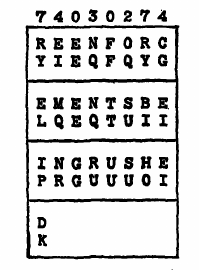
\includegraphics[width=0.3\textwidth, natwidth=199,natheight=270]{Chapter3_Figure17b.eps}
 \caption{Figure 17b}
\end{figure}

The cipher text is then transcribed in groups of five letters, reading
the successive lines in the normal manner, that is, from left to right and
from the top downwards, yielding the groups YIEQF, QYGLQ, etc. It is
no more difficult to encipher a message by this systematized procedure
than by the longer and slower method of writing the text out in long
lines and repeating the key over and over again. What is more important
is that the shortened procedure promotes accuracy in enc1pl'1erment. A
few seconds careful checking of the relative positions in which the two
alphabet strips are set is all that is required but this checking is very'
necessary, for if that is wrong all the cipher letters in that column to
which this setting applies will be in error.

\subsection{Using Key Words to Indicate Number, Identity, and Sequence of Cipher Alphabets Employed}

\mypara If reference is made to the two settings of alphabet strips in paragraph 58, it will be noted that in the first setting A\textsubscript{\textit{p}} = H\textsubscript{\textit{c}}, in the second
A\textsubscript{\textit{p}} = E\textsubscript{\textit{c}}. If the eight settings of the strips are studied it will be found
that the letters which A\textsubscript{\textit{p}}, represents successively are H, E, A, D, A, C,
H, and E, giving the word HEADACHE. These settings, when first
presented in the foregoing description, correspond merely to the numerical key 74030274, but this numerical key is also expressible in terms of
letters, which when put together properly spell a word. This is only
another way of showing that key words may be employed in this type of
substitution as in those previously described. Key words of various
lengths and composition may be used, consisting of single words, long
phrases, or sentences. In general, the longer the key the greater is the
degree of cryptographic security. The method as a whole is often
referred to as the repeating lacy method.

\mypara The number of elements in the key—that is, the number of letters
or figures composing it——determines the number of alphabets to be employed. The identity of each element of the key, the specific letter or
figure it happens to be, determines specifically which of a set of cipher
alphabets pertaining to the whole system will be used. And the specific
sequence or relative order of the elements of the key determines spe-
cifically the sequence with which the cipher alphabets are employed within the encipherment. The total number of cipher alphabets pertaining to
or composing the system may be limited or unlimited. When they are
produced as a result of the sliding of two basic or primary alphabets
against each other, the number is limited to 26 in the English alphabet.

\mypara A brief notation for indicating or designating a specific key letter
is to suffix the subscript “k” to it, just as the subscripts “p” and “c”
are suffixed to letters to indicate letters of the plain text or cipher text,
respectively. When the key letter occurs in an equation, it can be en-
closed within parentheses to avoid ambiguity. Thus, B\textsubscript{\textit{p}} (D\textsubscript{\textit{k}}) = E\textsubscript{\textit{c}}
means that plain-text letter B when enciphered by key letter D (in a
certain alphabet system) yields the cipher letter E.

\subsection{Use Of Other Types of Alphabets}

\mypara It has been noted that in the case of monoalphabetic ciphers, alphabets of various types may be employed. This is likewise true of polyalphabetic ciphers. Instead of using two alphabet strips bearing the
normal alphabetic sequence to determine the cipher equivalent of a letter
enciphered by a given key number or key letter, one may use a pair of
strips, one of which bears the normal direct, the other the normal reversed
sequence. In the former case one is dealing with direct' standard, in the
latter, with reversed standard alphabets.

\mypara Polyalphabetic substitution with direct or reversed standard alphabets does not result in nearly so great a degree of cryptographic security
as that resulting from the simple artifice of providing mixed alphabets
for the strips. All sorts of mixed alphabets may be used. One of the
strips may bear the normal direct or reversed sequence; the other a
mixed sequence. Both strips may bear identical mixed sequences proceeding in the same direction, or in opposite directions. Finally, both strips
may bear different mixed sequences.

\mypara In all cases, except where reciprocal alphabets are produced, it is
essential that the correspondents agree upon the sequence or strip from
which the plain and the cipher letters respectively will be taken, that is,
it is necessary to indicate which sequence constitutes the plain component, which the cipher component. If this is not done, two correspond-
ents will have difl‘iculty in deciphering one another’s messages. Also, as
noted above, it is necessary to agree as to which letter the key letter is to
be set against. The usual method is to agree that the initial letter of the
plain component, usually Ap, will be set opposite the key letter, though
other conventions are possible.

\mypara The sequences on the strips may be permanent or invariable, but
naturally the degree of cryptographic security in this case is considerably
lower than if they can be changed easily at the will of the correspondents
and by prearrangement. It is possible that a secret word may serve as
the basis not only for the key for shifting the strips, but also for the
mixing of the alphabetic sequences. For example, two correspondents
may agree to use the key CENTRAL AMERICA; to use the first part
as the basis for constructing the mixed plain component; the second part,
for constructing the cipher component; and to use the whole phrase as
the key for enciphcring the message. All the methods of constructing systematically mixed alphabets as described in section III of this chapter
are applicable.

\section{CIPHER DISKS AND SQUARE TABLES}
\subsection{Cipher Disks}

\mypara In the foregoing section it was noted that the separate alphabets
employed in the encipherment are produced by the use of only two strips
of paper bearing the normal alphabet. Such strips are often referred to
as sliding alphabets, because they can be shifted or slid against each other
in any one of 26 points of contact or coincidence. Exactly the same
results, so far as cipher equivalents are concerned, can be obtained by the
use of other devices. First, there are the so-called cipher wheels or cipher
disks in which an alphabet is written on the periphery of a rotating disk,
the circumference of which is divided into 26 equal segments, and this
disk is made to revolve concentrically upon a similar but slightly larger
fixed disk. Figure 18 shows the now obsolete U. S. Army Cipher Disk,
which is of this simple type. Here the alphabetic sequences are printed
on glossy celluloid, are permanent, and admit of no variatiom The
use of unglazed celluloid upon which blank segments appear would
permit of writing letters and erasing them as often as desirable. Thus,
quick and easy change of alphabets would be possible.

\begin{figure}[h]
 \centering
 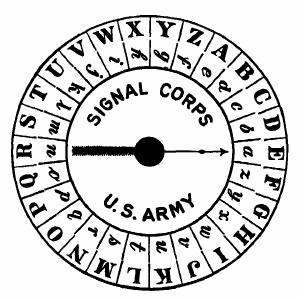
\includegraphics[width=0.6\textwidth, natwidth=303,natheight=298]{Chapter3_Figure18.eps}

        {\centering
        \small{\textit{To encipher a message, the key letter or the first letter of the
key word or phrase is set opposite “a.” Let us assume it
to be "E." The cipher letters to be written are those
opposite the text letter when “a" on the circle is set
opposite "E” on the card. For example, “send powder"
would be written "MARBPQIBAN." To use a key word
or phrase, each letter is used in turn to encipher one letter
only. When the last letter of the key word is used, repeat
until all letters of the message are enciphered. Numbers
when enciphered with the disk must be spelled out.}}
\par }
 \caption{Figure 18}
\end{figure}

\mypara The cipher alphabetsproduced by the cipher disk shown in the
figure are merely reversed standard alphabets, the same as are produced
by the use of sliding strips of paper, and by the use of certain; tables
which are discussed below. The method of employing the disk needs no
discussion. It may serve in monoalphabetic or polyalphabetic substitution
with a key word or key number.

\subsection{Square Tables}

\mypara Tables known in the literature of cryptography under various
names, such as “Vigenére Table", "Square Table”, "Quadricular Table”,
”Pythagorean Table”, “Cipher Square”, “Cipher Chart", etc., are often
employed in polyalphabetic substitution. All the results produced by their
use can be duplicated by the employment of sliding alphabets or revolving disks. The modern form of the Vigenére Table is shown in figure 19.
Such a table may be used in various ways, difl‘ering from one another in
minor details. The most common method is to consider the top line of
the table as containing the plain-text letters, the first column at the left
as containing the key letters. Then each successive horizontal line con-

\begin{figure}[h]
 \centering
 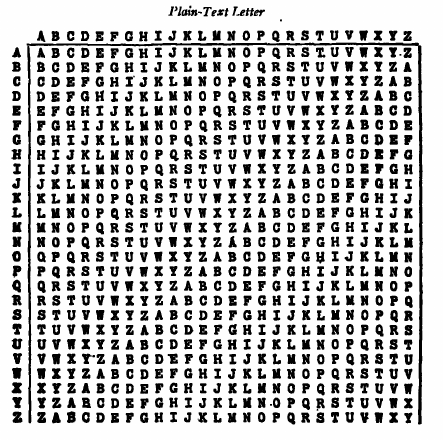
\includegraphics[width=0.8\textwidth, natwidth=443,natheight=440]{Chapter3_Figure19.eps}
 \caption{Figure 19. The Vigenere Table.}
\end{figure}

 

tains the cipher equivalents for the plain-text sequence ABC . . . Z enciphered by the key letter which stands at its left in the first column.
Thus, the cipher alphabet corresponding to key letter D is the sequence
of letters in the fourth horizontal line under the plain-text line, where
A, = Dc, Bp = EC, etc. It will be easy to remember, in using such a
table, that the equivalent of a given plain-text letter, T,,, for example,
enciphered by a given key letter, 0);, lies at the intersection of the vertical
column headed by T, and the horizontal row begun by O. In this case
Tp (0k) = He. The same result will be found on referring to sliding,
direct standard alphabets.

\mypara Minor modifications of the Vigenere Table are encountered. If the
top line is made a reversed normal sequence, leaving the interior of the
table unchanged, or if the successive horizontal rows are made to contain
the reversed normal sequence, leaving the top row (plain text) unchanged, then the results given by using the table are the same as those
given by using the obsolete cipher disk shown in figure 18. Again, the
same general results can be obtained by using a set of alphabets in tabular form known under the names of Porta’s Table and Napoleon’s Table,
which is ShOwn in figure 20.

AB ABC.DEFGHIJKLM
NOPQRSTUVWXYZ
CD ABCDEFGHIJKLM
ZNOPQRSTUVWXYZ
EF ABCDEFGHIJKLM
YZNOPQRSTUVWX
etc.
WX ABCDEFGHIJKLM
PQRSTUVWXYZNO
YZ ABCDEFGHIJKLM
OPQRSTUVWXYZN

figure 20

In this table the alphabets are all reciprocal, for example, G, (W\textsubscript{\textit{k}}) = V\textsubscript{\textit{c}},
V\textsubscript{\textit{p}} (W\textsubscript{\textit{k}}) = G\textsubscript{\textit{c}}. Reciprocal alphabets when arranged in this form are
sometimes called complementary alphabets. Note that in each alphabet
either of two letters may serve as key letter indifferent1y: G\textsubscript{\textit{p}} (W\textsubscript{\textit{k}}) or
G\textsubscript{\textit{p}} (X\textsubscript{\textit{k}}) = V\textsubscript{\textit{c}}.

\mypara Another modification of the basic table, and one that employs numbers instead of letters as cipher equivalents is shown in figure 21. Since
many more than 26 different equivalents are available (100 pairs of
digits from 00 to 99, it is possible to insert many plain—text elements in
 

 

 

 

abodefghi

jklmnopqr

It

stuvwxy:

0123456789

 

u'<u£<ceuna'uoDEU-I'H-wlrmnannvh

10 11 12 13 14 15 16 17 18
11 12 13 14 15 16 17 18 19
12 1314 1516 17 18 19 20

13 14 1516 17 18 I9 20 21 -

14 15 16 17 18 19 20 21 22
15 i6 17 18 19 20 21 22 23
16 17 18 19 20 21 22 23 24
17 18 19 20 2122 23 24 25
18 19 20 21 22 23 24 25 26
19 20 21 22 23 24 25 26 27
20 21 22 23 24 25 26 27 28
21 22 23 24 25 26 27 28 29
22 23 24 25 26 27 28 29 30
23 24 25 26 27 28 29 30 31
24 25 26 27 28 29 30 31 32
25 26 27 28 29 30 31 32 33
26 27 28 29 30 31 32 33 34
27 28 29 30 31 32 33 34 35
28 29 30 31 32 33 34 35 36
29 30 31 32 33 34 35 36 37
30 31 32 33 34 35 36 37 38
31 32 33 34 35 36 37 38 39
32 33 34 35 36 37 38 39 40
33 34 35 36 37 38 39 40 41
3435363738394041 42
35363738394041 4243

uwu£<=nu~avn=awrwmrmman-awn

19 20 21 22 23 24 25 26 27
20 21 22 23 24 25 26 27 28
21 22 23 24 25 26 27 28 29
22 23 24 25 26 27 28 29 30
23 24 25 26 27 28 29 30 31
24 25 26 27 28 29 30 31 32
25 26 27 28 29 30 31 32 33
26 27 28 29 30 31 32 33 34
27 28 29 30 31 32 33 34 35
28 29 30 3132 33 34 35 36
29 30 31 32 33 34 35 36 37
30 31 32 33 34 35 36 37 38
31 32 33 34 35 36 37 38 39
32 33 34 35 36 37 38 39 40
33 34 35 36 37 38 39 40 41
34 35 36 37 38 39 40 41 42
35 36 37 38 39 40 41 42 43
36 37 38 39 40 41 42 43 44
37 38 39 40 41 42 43 44 45
38 39 40 41 42 43 44 45 10
39 40 41 42 43 44 45 10 11
40 41 42 43 44 45 10 11 12
41 42 43 44 45 10 11 12 13
42 43 44 45 10 11 12 13 14
43 44 45 10 11 12 1314 15
44 45 10 11 12 13 14 15 16

u'<a£<=ou-u.a'uosBaku-i-a'wnoaac'p

28 29 30 31 32 33 34 35
29 30 31 32 33 34 35 36
30 31 32 33 34 35 36 37
31 32 33 34 35 36 37 38
32 33 34 35 36 37 38 39
33 34 35 36 37 38 39 40
34 35 36 37 38 39 40 41
35 36 37 38 39 40 41 42
36 37 38 39 40 41 42 43
37 38 39 40 41 42 43 44
38 39 40 41 42 43 44 45
39 40 41 42 43 44 45 10
40 41 42 43 44 45 10 11
41 42 43 44 45 10 11 12
42 43 44 45 10 1112 13
43 44 45 10 11 1213 14
44 45 10 11 1-2 13 14 15
45 10 11 12 13 14 15 16
10 11 12 13 14 15 16 17
1112 13 14 15 16 17 18
12 13 1415 16 17 18 19
13 1415 16 17 18 19 20
14 1516 17 18 19 20 21
15 16 17 18 19 20 21 22
16 17 18 19 20 21 22 23
17 18 19 20 21 22 23 24

an:xa<=nnnnvo=B—ru-wrn-onaup

36 37 38 39 40 4142 43 44 45
37 38 39 40 41 42 43 44 45 10
38 39 40 41 42 43 44 45 10 11
39 40 41 42 43 44 45 1011 12
40 41 42 43 44 45 101112 13
41 42 43 44 451011 12 1314
42 43 44 45 101112 13 14 15
43 44 451011 1213 14 15. 16
44 45 101112131415 16 17
45 1011 1213 1415 16 17 18
10 11 12131415 16 17 18 19
1112 131415 16171819 20
12 131415 16 '17 18 19 20 21
13 141516 17 1819 20 21 22
14 15 16 17 18 19 20 21 22 23
15 16 17 18 19 20 21 22 23 24
16 17 18 19 20 21 22 23 24 25
17 18 19 20 21 22 23 24 25 26
18 19 20 21 22 23 24 25 26 27
19 20 21 22 23 24 25 26 27 28
20 21 22 23 24 25 26 27 28 29
21 22 23 24 25 26 27 28 29 30
22 23 24 25 26 27 28 29 3D 31
23 24 25 26 27 28 29 30 31 32
24 25 26 27 28 29 30 31 32 33
25 26 27 28 29 30 31 32 33 34

awx¢<caannuoua—rwu-rnnanaa‘r

 

 

 

nbcdefghi

 

 

jklmnopqr

 

G

 

 

stuvwxyz

 

0123456789

 

Q

 

 

[.5

Figure

21.


the top line of the table in addition to the 26 letters. For example, one
could have the 10 digits; a few common double-letter combinations, such
as DD, LL, RR, SS; a few of the most frequently used pairs of letters,
such as TH, ER, IN, or even such common syllables as ENT, INC, and
ION

\subsection{Square Tables Employing Mixed Alphabets}

\mypara In the tables thus far shown the alphabets have been direct or
reversed standard sequences, but just as mixed sequences may be written
upon sliding strips and revolving disks, so can mixed alphabets appear in
tabular form. The table shown in figure 22, based upon the key word
sequence derived from the word LEAVENWORTH, is an example that
is equivalent to the use of a strip bearing the same key word sequence
sliding against another strip bearing the normal alphabet.

n.

uuxcmnmssunnuuouzawoaz<>uu>
runucmpwsxuunuunusawoaz<>nu
mrNnxcmomflwthmunumawoiz<>a
>mrnuxcmomgxuunmuau=awoaz<u
<>mrnnxcmpmuxuunuuaumawoazm
z<>mruuxdmpwifithnunumawoaw
==<>mruHucmpwzwuHhuunwmauon
0S2<>HFNHNGMSMIKQHQMUOU=HH=
uoaz<>mruuxcmpvsuunnuuoumau
anosz<>mru«xcmpmswuuaquawmh
mawoa=<>mruuxcmpvgxunannu:
wmawoaz<>mrunxqmpm=qunuuor
nu:amoaz<bmrNNNGMDVINthflUH
acumenoaz<>mruducmpu=nuunmz
muoumawo==<>mruuucmnwxnunno
anudumawoazd>mruuucmpmzaanw
Homeammaxoaz<>mruuucmpwswho
anonunumawoaz<>nruuucmavuau
uhnaqunu=awoaz<>nrnux:mnw:m
s:anuuaumaxoaz<>nruwucmowa
w:qunuunumawoaqumruuucmpc
onxauuawuaumawoiz<inrunucm<
mp1:xuunmunumauoazéfinrnuuc:
GmofiINQHfifiUOUIHNO‘Zd’flrflflufl
ucmomthnnuunu:auo:z<>urn«u
«aqua»:uhnéuuou=4uoazd>nrun

Figure 22.

The usual method of using such a table is the same as that in the preceding cases. The only difference is that the key letters must now be
s°ught in a mixed sequence, whereas in the preceding tables they were
located in normal direct or reversed sequences. Example, using figure 22:

C\textsubscript{textit{p}} (S\textsubscript{textit{k}}) = X\textsubscript{textit{c}}.


 

' ._ films-:14... _. .

H: I"._,455355;?“'lLi‘i-'w"ifi.'i"-‘S‘i“Li-1?" x- -:--.-.-,.c _---- -'- -_

ux=<xmgxh=nmun<rm>zonammco
onxa<wwzxu=nwuonrm>zOHammc
conxa<wm=xumnmuonrm>zouamu
HGDNxa<w1=Nu=nwun<rw>ZOHam
mmcouxa<wmsxu=nquonrm>zona
emmcpux=<ww=xh=nwunarw>zou
Hammconxa<mw=xh=nmuo«rw>zo
ouammcoNxa<ww=xumnman<ru>z
zOHammcouxs<wmzxumnwuomru>
>zonammconxa<wv=xu=nwunwru
m>zOHammcpNxa<mwzwu=nwunur
ru>20Hammcpwxa<xmth=ouunn
urm>zOHammcpNxa<xw==umnuon
aura»:0Hammcowxs<mmzuhxnuu
acarmszHammcpNasawwzwuznn
MUGKFW>ZOHHmmGDNNS<WflSNQZQ
QMUOKFW>ZOHHMMGDNNS<NVEXHI
Infidowfim>ZOHHMMGDNNS<N1=XQ
a:nmuoarw>zonemmcowxa<wwzx
an:embo<rw>20HammcpNxs<xmg
zxumnmunnnm>20Hammconx=<xm
manuxnwuonrw>zonammcpuxa<w
wmzxuznnconru>onammcouua<
<wv=xnmnuanmrw>zouammcnnxa
=<wvthmnwunnrw>2caammcnux
xa<wm:susnmoonrw>zonammcou

Figure 23.

\mypara Figure 23 illustrates a case in which a mixed alphabet is sliding
against itself. The usual method of employing such a table is exactly
the same as that explained before. The only difference is that both the
plain—text letters and the key letters must be looked for in mixed
sequences. Example, using figure 23: U\textsubscript{textit{p}} (R\textsubscript{textit{k}}) = V\textsubscript{textit{c}}.

\mypara It has been indicated that the basis of reference in most cryptographic operations involving key words is the letter A”. In employing
sliding alphabets it is usual to set the key letter as located in the cipher
component opposite the letter A as located in the plain component. But,
as shown in paragraphs 42!; and 60c, the key letter as located in the
cipher component is usually set opposite the initial letter of the plain
component. In all examples preceding that in figure 23, the key letter has
been A. In figure 23, since the plain component is also a mixed sequence
and its initial letter is Q, the sliding alphabets are set against each other
so that the given key letter in the cipher component is opposite Q in the
plain component. Thus, to duplicate the results given by the use of figure
23 in finding the value of Up (R1,), it is necessary to set the sliding strips
in the following relatiVe positions:

\begin{verbatim}
Plain: QUESTIONABLYCDFGHJKMNPRVWXZQUESTIONABLYCDEFGHJKM
Cipher:     QUESTIONABLYCDFGHJKMNPRVWXZ
\end{verbatim}

Here it is seen that U\textsubscript{textit{p}} (R\textsubscript{textit{k}}) = V\textsubscript{textit{c}}, which is identical with the, result
obtained from the use of the table. There are other ways of using the
table, however, each having a correspondingly modified method of employing sliding strips in order to obtain identical results.

\section{OBSERVATIONS ON CIPHER SYSTEMS}

\subsection{More Complex Substitution Systems}

\mypara The substitution systems discussed above are all based on relatively
simple methods. They can all be solved rapidly. More complicated systems have been devised, however, and are used in certain situations.
They are briefly described in this section.

\mypara Virtually all systems based upon the principle of a repeating key
can be solved because of certain cyclic or periodic phenomena, which the
use of a repeating key exhibits externally or internally in the cryptograms. There are methods for preventing the external manifestation in
the cryptograms of these phenomena, or their suppression and disguise
if present internally. In some, the principle is to make the elements of a
fixed or invariable-length key apply to variable or irregular-length groupings of the plain text so that no cyclic phenomena are exhibited by the
cryptograms. In others, the principle is to apply irregular lengths of the
key, or a variable-length key to regular and fixed groupings of the plain
text, with the same object in view. In still other methods, both principles
are combined, or the key itself is of such a nature that it does not repeat
itself. This may be brought about by constructing or establishing a non-repeating key, or by employing the key in a special manner. Systems in
which the successive letters of the cipher text or successive letters of the
plain text after the initial letter serve as successive key-letters are also
used with the object of avoiding or eliminating periodicity.

\mypara In the majority of the methods described the encipherment deals
with single letters, and is therefore monagraphit: in nature. There are,
however, certain methods in which encipherment is by pairs of letters,
called digraphic substitution, or by sets of three letters, called trigraphic
substitution. Polygraphic substitution methods, as they are mlled, have
for their object the suppression, so far as possible, of the characteristic
frequencies of individual letters, by means of which solution may be
reached. The methods may employ extensive tables, small squares,
rectangles, and other designs, or sets of sliding or rotating alphabets.
The Playfair C ipher, which was for many years a standard field cipher in
the British Army and was for a short time during World War I em—
ployed by the U. S. Army, is an example of digraphic substitution.

\subsection{Combined Substitution-Transposifion Systems}

In paragraph 10b, reference was made to the possibility of combining
within a single system both transposition and substitution methods; that
is, of first enciphering by a method of one type and then taking the re-
sulting cipher text and passing it through an encipherment of the other
type. The usual order is first to substitute and then to transpose, but
the reverse of this order of procedure is also possible. In some methods,
quite complex, there may be a first substitution, then a transposition, and
finally a substitution again. Despite the fact that three steps are in-
volved, certain of these systems may be practical for military use under
special conditions where speed is not as important as security. These
cannot be described in this manual.

\subsection{Cipher Devices and Cipher Machines}

\mypara Only a little practical experience with any of the methods described
is necessary to convince one that on the whole they are slow, more or less
cumbersome, and subject to errors that often delay or make impossible
the decryptographing of messages. Furthermore, from the point of view
of cryptographic security, when employed in regular voluminous traffiic
they leave much to be desired. Consequently, cryptographers, both experienced and inexperienced, have been led to attempt to devise ap-
paratus which will not only facilitate cryptographing and decryptographing, but will also increase the degree of cryptographic security. Small
instruments constructed for this purpose, operated by hand, are called
cipher devices. Scores of them have been devised, but only a few are
sufficiently practicable for field use, and still fewer are of such construction that they produce cryptograms of unusual security. Among the
better examples of such cryptographs is one which was for some years
(1922—42) employed in the U. S. Army under the name of Ciphef
Device, Type M—94. Modern security requirements made such a device
obsolete, however, and it has been replaced by a better one, the Converter
M-209 ( ) (TM 11—380).

\mypara There are larger cryptographic machines which are much more
nearly automatic in nature and can therefore be operated at a much
greater rate of speed. These are usually equipped with typewriter keyboards which can be manipulated with considerable speed; the machine
may also print the results of the enciphering or deciphering operations.
Sometimes they are equipped with electrical transmitters and can thus
serve not only to encipher and decipher messages but also to transmit
them automatically. A mechanism of the latter nature is usually in the
form of a modified printing telegraph machine, or else it consists of an
auxiliary piece of apparatus used in conjunction with the teleprinter.
Such apparatus can obviously be practicably employed only among the
larger headquarters where traffic is sufliciently heavy to warrant its use.

\subsection{Disadvantages and Limitations of Cipher Systems}

Except for certain electrically operated cipher machines equipped with
a typewriter keyboard, most cryptographic methods using “manual"
or “pencil and paper” cipher systems are unsatisfactory for military pur—
poses. Practically all such systems can be solved by enemy cryptanalysts,
and those suitable for use in the theater of operations offer fewer ob—
stacles to solution than systems suitable for use in the rear areas. Cipher
systems are not economical in time units required in electrical transmis-
sion; the best that they can do is to produce cryptograms no longer than
the original plain text. For use within small tactical units in the forward
areas there are other cryptographic methods which offer advantages of
speed, simplicity, and brevity and which, properly used, afford sufl’icient
cryptographic security. These are often preferred over cipher methods in
the forward echelons of the combat zone. These methods involve the use
of lists of groups of letters or figures to which arbitrary meanings have
been assigned. They are called “field codes,” “prearranged-message
codes,” “brevity codes,” “voice codes,” “jargon codes,” etc. Codes will
be discussed in the succeeding sections of this manual.
